\documentclass[border=3pt]{standalone}
\usepackage{tikz}
\usetikzlibrary{patterns}
\begin{document}
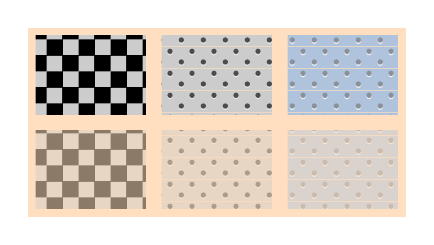
\begin{tikzpicture}
\fill[orange!25] (-.1,-.1) rectangle (4.7,2.3);
\fill[pattern=checkerboard light gray,pattern color=red] (0,1.2) rectangle (1.4,2.2);
\fill[pattern=crosshatch dots gray,pattern color=red] (1.6,1.2) rectangle (3,2.2);
\fill[pattern=crosshatch dots light steel blue,pattern color=red] (3.2,1.2) rectangle (4.6,2.2);
\fill[pattern=checkerboard light gray,pattern color=blue,fill opacity=.45] (0,0) rectangle (1.4,1);
\fill[pattern=crosshatch dots gray,pattern color=blue,fill opacity=.45] (1.6,0) rectangle (3,1);
\fill[pattern=crosshatch dots light steel blue,pattern color=blue,fill opacity=.45] (3.2,0) rectangle (4.6,1);
\end{tikzpicture}
\end{document}
